\documentclass{zjureport-zh}

\major{计算机科学与技术}
\course{并行计算与多核编程}
\name{陈卓}
\expname{并行矩阵乘法设计}
\stuid{3170101214}
\instructor{楼学庆}
\college{计算机科学与技术学院}
\title{并行计算与多核编程}

\usetikzlibrary{positioning}
\tikzset{state/.style = {draw=black,circle}}
\tikzset{arrow/.style = {->,thick}}


\begin{document}

\makecover

%\maketitle

\section{设计原理}
\par 本实验分别采用 Cannon 算法和 DNS 算法实现 $4 \times 4$ 矩阵乘法。

\subsection{Cannon 算法} \label{cannon}
\par 对于 $N \times N$ 矩阵乘法 $A \times B$,本实验 Cannon 算法采用\textbf{二维网孔结构}。步骤如下:
\begin{enumerate}[label=\roman*), itemindent=2em]
	\item $A_{ij}$ 向左循环移动 $i$ 步;$B_{ij}$ 向上循环移动 $j$ 步\footnote{$i,j \in [0,N)$};各结点清零; \label{cannon1}
	\item 各结点做乘法运算并累加;\label{cannon2}
	\item $A_{ij}$ 向左循环移动 1 步;$B_{ij}$ 向上循环移动 1 步;\label{cannon3}
	\item 重复 $N-1$ 次。
\end{enumerate}

\subsection{DNS 算法}


\section{设计思路与实现}

\subsection{Cannon 算法}
\par 根据 \ref{cannon} 中的描述,本实验将 $4 \times 4$ 矩阵分块为 16 个结点,每个结点处理两个数的乘法运算。
\subsubsection{cannon\_unit 模块}
\par 首先设计出表达每个结点的 \texttt{cannon\_unit} 模块。
\begin{lstlisting}[language=verilog]
module cannon_unit(
	input wire clk,
	input wire rst,
	input wire en,
	input wire a_init[7:0],
	input wire b_init[7:0],
	input wire a_in[7:0],
	input wire b_in[7:0],
	output wire a_out[7:0],
	output wire b_out[7:0],
	output reg s[7:0]
);
\end{lstlisting}
\par 其中 \texttt{rst, a\_init, b\_init} 用于步骤 \ref{cannon1} 的初始化和清零;\texttt{a\_in, b\_in, a\_out, b\_out} 用于在二维网孔结构中连接其它结点;\texttt{s} 用于输出;\texttt{en} 用于计算完成后阻断后续计算。
\par 在 \texttt{cannon\_unit} 模块中有三个寄存器 \texttt{a, b, s},分别用于保存 $A,B$ 矩阵的元素和结果。在每个时钟周期内,寄存器 \texttt{a, b} 接收来自输入 \texttt{a\_in, b\_in} 的值,同时将二者乘积累加在 寄存器 \texttt{s} 中;若 \texttt{rst} 置位,则 \texttt{s} 清零,\texttt{a, b} 接收 \texttt{a\_init, b\_init} 的值。

\subsubsection{cannon 模块}
\par \texttt{cannon} 模块是一个状态机。根据 Cannon 算法设计 4 个状态,分别是 \texttt{IDLE, LOAD, CALC, END}。状态转移如\figref{cannon_statefig} 所示。

\begin{lstlisting}[language=verilog]
module cannon(
	input wire clk,
	input wire rst,
	input wire A[3:0][3:0][7:0],
	input wire B[3:0][3:0][7:0],
	output wire S[3:0][3:0][7:0],
	output reg finished
);
\end{lstlisting}

\begin{figure}[h]
	\centering
	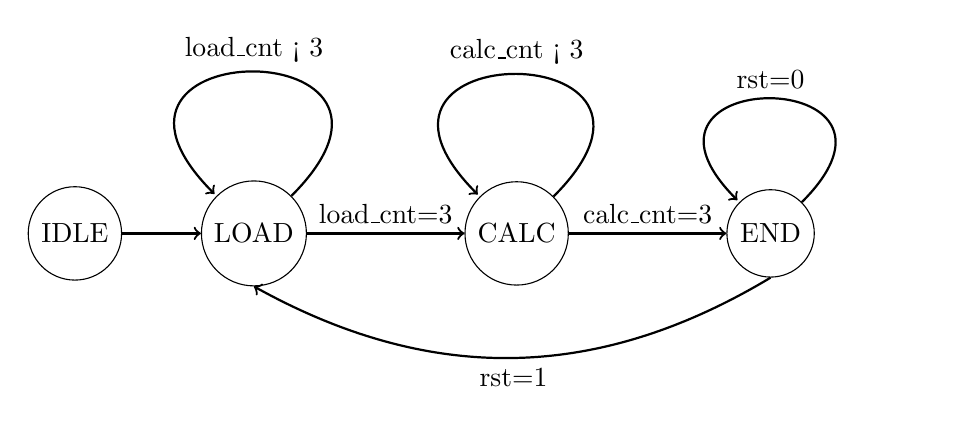
\begin{tikzpicture}
		\node[state] (idle) {IDLE};
		\node[state, right=of idle] (load) {LOAD};
		\node[state, right=2 of load] (calc) {CALC};
		\node[state, right=2 of calc] (end) {END};
		\path[arrow] (idle) edge (load);
		\path[arrow] (load) edge [loop] [above] node {load\_cnt < 3} (load);
		\path[arrow] (load) edge [above] node {load\_cnt=3} (calc);
		\path[arrow] (calc) edge [loop] [above] node {calc\_cnt < 3} (calc);
		\path[arrow] (calc) edge [above] node {calc\_cnt=3} (end);
		\path[arrow] (end) edge [loop] [above] node {rst=0} (end);
		\path[arrow] (end.south) edge [bend left] [below] node {rst=1} (load.south);
	\end{tikzpicture}
	\caption{\texttt{cannon} 模块状态图} \label{cannon_statefig}
\end{figure}

\par 每个状态的动作如\tabref{cannon_statetab} 所示。
\begin{table}[h]
	\centering
	\caption{\texttt{cannon} 模块状态表} \label{cannon_statetab}
	\vspace{1ex}
	\begin{tabular}{cc}
		\hline
		状态 & 描述 \\
		\hline
		\texttt{IDLE} & 模块初始化 \\
		\hline
		\texttt{LOAD} & \makecell{加载 $A,B$ 矩阵,\\并初始化各结点} \\
		\hline
		\texttt{CALC} & 循环位移计算 \\
		\hline
		\texttt{END} & 计算结束 \\
		\hline
	\end{tabular}
\end{table}

\par 详细代码见 \texttt{cannon.v}。

\section{评价}
\subsection{Cannon 算法}
\par 设 $k^2$ 个结点,记单次传输时间 $t_r$,单次计算时间 $t_w$,由于步骤 \ref{cannon2} 和 \ref{cannon3} 同时进行,且通常 $t_r << t_w$,故总时间
$$
	T = (k-1)t_r + kt_w
$$
\par 此外,若单个结点中分块矩阵的乘法采用串行算法,则
\begin{align*}
	T &= (k-1)O(1) + kO((\frac{n}{k})^3) \\
	  &= O(k) + O(\frac{n^3}{k^2}) \\
	  &= O(\sqrt{p}) + O(\frac{n^3}{p}) \\
	  &= O(\frac{n^3}{p})
\end{align*}
\par 在本实验中,每个结点仅负责一阶矩阵的运算,故 $T = O(\sqrt{p})$。
\par Cannon 算法的不足之处在于,数据初始化需要 $k-1$ 次的循环位移,在本实验中,由于规模不大,可以通过直接在代码中交换输入实现加速,但在大规模矩阵运算中仍然有这一方面的劣势。

\subsection{DNS 算法}


\section{$N \times N$ 矩阵乘法设计}
\subsection{Cannon 算法}
\par Cannon 算法是容易推广的——尽管本实验每个结点仅处理两个数的运算,但在实际使用中可以令每个结点处理两个小矩阵的运算,即 Cannon 算法描述中的\textbf{分块}。然而如此一来,如何对大矩阵进行分块,分块方式不同对运算复杂度是否有影响,就成为应该思考的问题。此外,本实验使用 verilog 设计 $4 \times 4$ 矩阵乘法,而对于高阶矩阵乘法,我们为它不可能设计新的硬件,应该以小模块为基础,利用高层的并行算法(如 MPI)实现高阶矩阵乘法。
\par 假设已有用 Cannon 算法处理 $S$ 阶矩阵乘法的结点 $P$。由于任何 $S'(<S)$ 阶矩阵,我们可以通过补零的方式用 $P$ 计算。因此对于 $N(>S)$ 阶矩阵,我们可以将其补成 $N'$ 阶矩阵,其中
$$
	N' = \lceil\frac{N}{S}\rceil S = kS
$$
\par 此时通过使用 $k^2$ 个 $P$ 结点,就可以组成更高层的 Cannon 算法(称为\textbf{法一})。下面与硬件直接实现的 $N$ 阶矩阵乘法(称为\textbf{法二})比较。
\par 记循环移动的次数、乘法累加的周期数分别为 $r, w$。设法一不同结点之间的带宽是 $S$ 阶矩阵的大小,则需要 $k$ 个周期初始化移动;接下来的 $k-1$ 次循环移动计算中,每次都需要 $P$ 结点内 $S$ 个周期初始化,并有 $S-1$ 次结点内的循环移动计算。则有
\begin{align*}
	r_1 &= k-1 + k(2S - 1) \\
		&= 2N' - 1 \\
	w_1 &= kS \\
		&= N' \\
	r_2 &= 2N-1 \\
	w_2 &= N
\end{align*}

\par 从以上可以看出,使用法一所带来的性能损失仅为 $O(S)$,因此我们可以使用法一扩展 Cannon 算法。

\subsection{DNS 算法}



\end{document}
















